\documentclass[english]{article}
\usepackage[latin9]{inputenc}
\usepackage{graphicx}
\usepackage{babel}

\usepackage{verbatim}
\usepackage{array}
\usepackage{bbm}
\usepackage{amsthm,amssymb,amsbsy,amsmath,amsfonts,amssymb,amscd,amstext}
\usepackage{dsfont}
\usepackage[top=2.5cm, bottom=2.5cm, left=3cm , right=3cm]{geometry}

\title{Exam solutions: Statistical modeling and its applications} %\\ \vspace{\baselineskip} %\null \\
%\Large{Processus gaussiens et mod�les de krigeage}}
\author{Mines St-Etienne -- 21st January 2015}
\date{}

\begin{document}

\maketitle
\vspace{-5mm}

\subsection*{Exercise 1 (5 pts)}
On consid\`ere la fonction $f(x_{1},x_{2})=e^{x_{1}}x_{2}$. On souhaite
r\'ealiser une analyse de sensibilit\'e globale de $f(X_{1},X_{2})$ lorsque
$X_{1}$ et $X_{2}$ sont des variables al\'eatoires ind\'ependantes uniformes
sur {[}-1/2, 1/2{]}.
\begin{enumerate}
\item Par sym\'etrie de la densit\'e de la loi unforme sur [-1/2, 1/2] on a $E(X_{2})=0$. %D'autre part $m_{1}:=E(e^{X_{1}})=\int_{-1/2}^{1/2}e^{x_{1}}dx_{1}=e^{1/2}-e^{-1/2}$. 
\item Il y a deux m\'ethodes possibles ici, soit calcul direct, soit proposer une d\'ecomposition et v\'erifier qu'elle satisfait les hypoth\`eses d'ind\'ependances et de non-simplification (voir TDs). 
On obtient\\
 $\mu_{0}=0$, $\mu_{1}(x_{1})=0$, $\mu_{2}(x_{2})=m_{1}x_{2}$, $\mu_{1,2}=(e^{x_{1}}-m_{1})x_{2}$
\item \_

\begin{enumerate}
\item En utilisant l'ind\'ependance de $X_{1}$ et $X_{2}$, on a $\text{var(}f(X_{1},X_{2}))=E((e^{X1})^{2})E(X_{2}^{2})=(m_{1}^{2}+v_{1})v_{2}$ 
\item $S_{1}=0$ est \'evident. $D_{2}=\text{var}(\mu_{2}(X_{2}))=m_{1}^{2}v_{2}$
d'o\`u l'expression attendue. 
\item La somme des indices de Sobol vaut 1 donc $S_{1,2}=1-S_{2}=\frac{v_{1}}{m_1{^{2}}+v_{1}}$.
\end{enumerate}
\end{enumerate}


\subsection*{Exercise 2 (3 pts)}
\begin{enumerate}
\item $X_{2},X_{3},X_{5}$ sont sont influentes (hi\'erarchie : $X_{2},X_{5},X_{3}$)
; les autres n'inter-viennent pas du tout car leur effet total est
nul. $X_{2}$ interagit avec les variables influentes, donc seulement avec $X_{3}$
et $X_{5}$ (le graphique ne permettant pas d'aller plus loin). Les
variables individuelles expliquent 80\% de la variance, le reste \'etant
des interactions. 
\item Question de cours. Il faut dans l'ordre \'evaluer $f$ aux simulations,
ce qui donne un vecteur $y$ de taille $N$. Sa moyenne donne une
estimation de $\mu_{0}$. On repr\'esente ensuite $y-\mu_{0}$ contre
$x_{2}$ et on effectue un lissage, ce qui donne une estimation (moyenne
mobile, splines, polynomes locaux) de $E(f(X_{1},...,X_{8})\vert X_{2})-\mu_{0}$.\end{enumerate}


\subsection*{Exercise 3 (5 pts)}
\begin{enumerate}
\item Given the smoothness of the mean predictor, which is a linear combination of $k(x,X)$, the kernel could be squared exponential or Matern 5/2.
\item The smallest lengthcales ($\theta = 0.05$) can definitely be observed in the direction $x_1$ for the model $m_1$ since the model comes back very quickly to a mean value. Furthermore, the model $m_2$ seems to be isotropic, which is consistent with $(\theta_1,\theta_2)=(0.25,0.25)$ for this model.
\item Let $\mu$ and $C$ be the predicted mean values and covariance matrix for the test-set according to the model:
\begin{equation*}
 	\begin{split}
 		\mu & =k(X_{test},X)k(X,X)^{-1}F \\
 		C & = k(X_{test},X_{test}) k(X_{test},X)k(X,X)^{-1}k(X,X_{test}).
 	\end{split}
 \end{equation*} 
The standardised residuals $R$ are given by: $R = C^{-1/2} (F_{test} - \mu)$, where $C^{-1/2}$ is given, for example by the inverse of the Cholesky decomposition of $C$.

\item The second model should be preffered to the first one for two reasons : 
\begin{itemize}
	\item Its standardised residuals are actually close to a standart Gaussian distribution
	\item It has a better $Q_2$.
\end{itemize}

\item The first model comes back to a constant value (not equal to zero) when it is far from the observations, so there is a constant mean. Since we don't know the actual value of the variance parameter, it is not possible to say if the confidence intervals include an extra term accounting for the variance of the trend estimate. We thus don't know if it has been estimated or not.
\end{enumerate}

\subsection*{Exercise 4 (2 pts)}
\begin{itemize}
	\item $Z_1$ has a Matern 3/2 kernel with variance $\sigma^2 = 1$ and lengthcale $\theta = 0.2$
	\item $Z_2$ has a composite kernel which is a sum of a Gaussian kernel ($(\sigma^2,\theta) = (1.2)$ and a white noise kernel with a small variance ($\sigma^2 = 0.01$).
	\item $Z_3$ has a Brownian motion kernel with variance $\sigma^2 = 1$.
	\item $Z_4$ has a kernel of the shape constant plus linear : $\sigma_0^2 + \sigma_1^2 xy$, with $\sigma_0^2=0.05$ and $\sigma_1^2=1$.
\end{itemize}

\subsection*{Exercise 5 (3 pts)}
\paragraph{}
% ANOVA kernels over $\mathds{R}^d \times \mathds{R}^d$ are kernels of the form: $\displaystyle k_{anova}(x,y) = \sigma^2 \prod_{i=1}^d (1 + k_i(x_i,y_i)) $, where the $k_i$ can be any kernel over $\mathds{R} \times \mathds{R}$.

\begin{enumerate}
\item Since $(x,y) \mapsto 1$ is a valid covariance function, $k_{anova}$ can be seen as the sums and product of covariance functions. It is thus also a valid kernel.
\item Expanding the kernel expression gives
\begin{equation*}
 		k_{anova}(x,y) = \sigma^2 \left(1 + \sum_{i=1}^d k_i(x_i,y_i) + \sum_{i=1}^d \sum_{i=1}^d k_i(x_i,y_i) k_j(x_j,y_j) + \dots + \prod_{i=1}^d k_i(x_i,y_i) \right)
 \end{equation*} 
If we plug this in the best predictor expression, we obtain 
 \begin{equation*}
 	\begin{split}
 		m(x) & =k_{anova}(x,X)k_{anova}(X,X)^{-1}F \\
 		 & = \sigma^2 \left(1 + \sum_{i=1}^d k_i(x_i,X_i) %+ \sum_{i=1}^d \sum_{i=1}^d k_i(x_i,X_i) k_j(x_j,X_j) 
 		 + \dots + \prod_{i=1}^d k_i(x_i,X_i) \right) k_{anova}(X,X)^{-1}F \\
 		 & = m_0 + \sum_{i=1}^d m_i(x_i) + \sum_{i=1}^d \sum_{i=1}^d m_{i,j}(x_i,x_j) \dots + m_{1 \dots d}(x)
 	\end{split}
 \end{equation*} 
where $m_0 = 1 k_{anova}(X,X)^{-1}F$, $m_i(x_i) = k_i(x_i,X_i) k_{anova}(X,X)^{-1}F$, etc. The decomposition of the kernels shows that $Z$ can be seen as the sum of independent GPs:
 \begin{equation*}
 		Z(x) = Z_0 + \sum_{i=1}^d Z_i(x_i) + \sum_{i=1}^d \sum_{i=1}^d Z_{i,j}(x_i,x_j) \dots + Z_{1 \dots d}(x)
 \end{equation*} 
Given this decomposition, the submodels can be interpreted as $m_I(x_I) = \mathrm{E} [Z(x_I) | Z(X)=Z]$ ($I$ can be any subset of index).
\item The difference between the above decomposition of $m$ in submodels and its Sobol-Hoeffding decompostion is that the $m_I$ do not necessarily integrate to zero. This can be acheved by choosing the univariate kernels $k_i$ as kernels generating sample paths that intergate to zero, as it has been discussed during the course. 
\end{enumerate}

\subsection*{Exercise 6 (2 pts)}
\paragraph{}
Let $\mathcal{H}$ be a RKHS of functions over $[0,1]$ such that the derivative evaluation in 0 : $L: f \mapsto f'(0)$ is continuous.
% \begin{equation*}
%  	\begin{split}
%  		L: \mathcal{H} & \longrightarrow \mathds{R} \\
%  		f & \longmapsto \frac{\mathrm{d} f}{\mathrm{d} x}(0)
%  	\end{split}
%  \end{equation*} 
%  is continuous.

\begin{enumerate}
\item Since it is already stated in the wording that $L$ is continuous, we just need to stress that computing a derivative is a linear operator in order apply the Riesz theorem:
 \begin{equation*}
 		L(f + \lambda g) =  \left. \frac{\mathrm{d}}{\mathrm{d} x} (f + \lambda g) \right |_0 =
 		\left. \frac{\mathrm{d} f}{\mathrm{d} x} \right |_0 + 
 		\left. \lambda \frac{\mathrm{d}g}{\mathrm{d} x} \right |_0 
 		= L(f) +  \lambda L(g)
 \end{equation*} 
 Let $r$ be its Riesz representer: Since $r \in \mathcal{H}$, we have $r(x) = \langle r, k(x,.) \rangle_\mathcal{H} = L(k(x,.)) = \frac{\mathrm{d} k(x,s)}{\mathrm{d} s}(0)$.
\item The subspace $\mathcal{H}_0$ corresponds to the subspace orthogonal to $r$ so we have $k_0 = k - k_r$ where $k_r$ is the reproducing kernel of $Span(r)$. Furthermore, the expression $k_r$ is:
 \begin{equation*}
 		k_r(x,y) = \frac{r(x) r(y)}{r'(0)}
 \end{equation*} 
\end{enumerate}

\end{document}
























\subsection*{Exercise 1 (2014 exam)}
\paragraph{}
The graphs bellow show samples of centred Gaussian process. What kernel may have been used to generate these figures? Justify briefly your answer.
\begin{figure}[!ht]%
\begin{center}
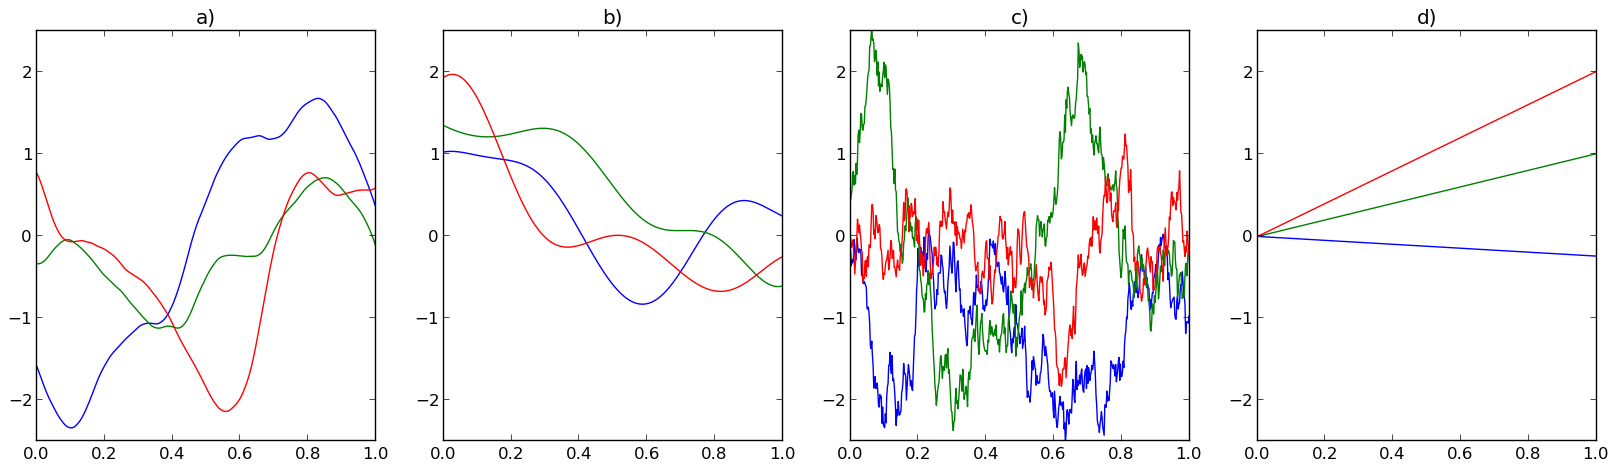
\includegraphics[width=\textwidth]{python/Ex1}
\end{center}
\end{figure}

%%%%%%%%%%%%%%%%%%%%%%%%%%%%%%%%%%%%%%%%%%%%%%%%%%%%%%%%%%%%%%%%%%%%%%%%%%%%%%%%
\subsection*{Exercise 2 (2014 exam)}
For the four models bellow, indicate:
\begin{itemize}
	\item the type of trend that is considered
	\item if the trend is known or estimated
	\item the kernel used
	\item if there is observation noise
\end{itemize}

\begin{figure}[!ht]%
\begin{center}
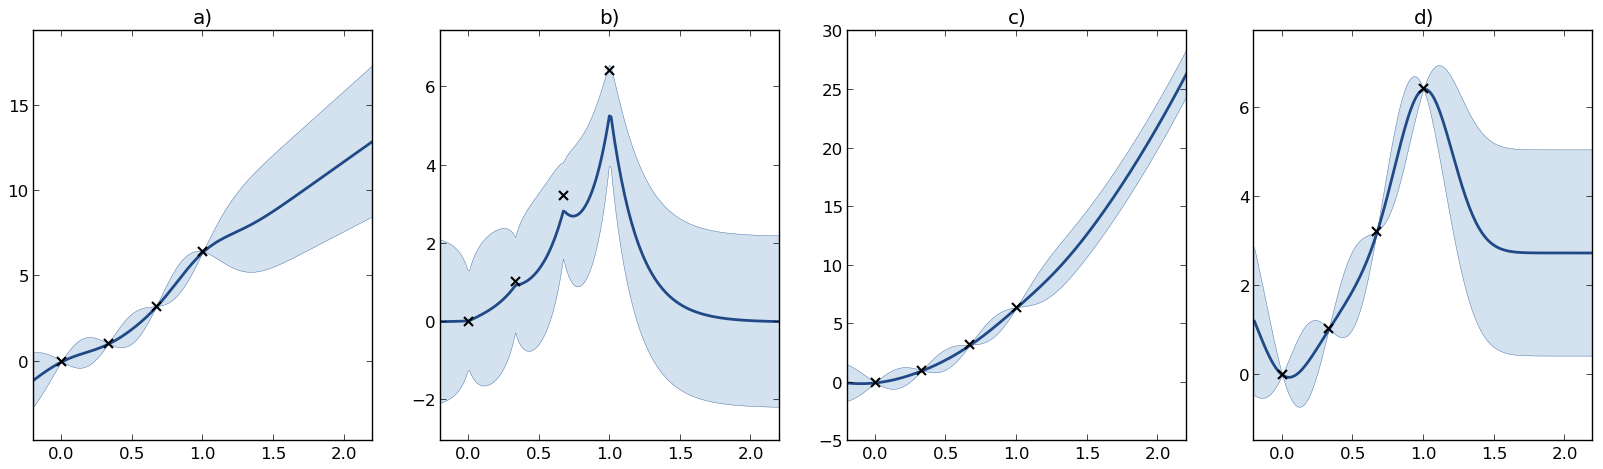
\includegraphics[width=\textwidth]{python/Ex2}
\end{center}
\end{figure}
Suggest a model that would be suited to the data at hand.

%%%%%%%%%%%%%%%%%%%%%%%%%%%%%%%%%%%%%%%%%%%%%%%%%%%%%%%%%%%%%%%%%%%%%%%%%%%%%%%%
\subsection*{Exercise 3 An alternative to ordinary kriging}
An alternative to kriging model with trend is to consider sums of kernels where some of the kernels correspond either to the space generated by basis functions or to spaces of low frequency functions. Let $X$ be a $\mathcal{N}(0,s^2)$ random variable and let $Z_1$ be the random process defined by $Z_1(x) = 1 \times X$.

\paragraph{1.} Prove that $Z_1$ is a Gaussian process. Give the expressions of it's mean $m_1$ and covariance $k_1$. 

\paragraph{2.} What happen if we try to build a Gaussian process regression model based on $Z_1$.

\paragraph{3.} Let $Z$ be a centered Gaussian process with kernel $k_Z$. We define a new GP $Y(x) = Z(x) + Z_1(x)$ where $Z$ and $Z_1$ are taken independently. What is the covariance of $Y$ ? 

\paragraph{4.} Give the expression of the Gaussian process model based on $Y$. Show that the best predictor can be written
\begin{equation*}
	m(x) = \frac{\mathbf{1}^t K^{-1} F}{1/s^2 + \mathbf{1}^t K^{-1} \mathbf{1}} + k(x,X) K^{-1} \left( F - \mathbf{1} \frac{\mathbf{1}^t K^{-1} F}{1/s^2 + \mathbf{1}^t K^{-1} \mathbf{1}} \right)
\end{equation*}
where $K = k(X,X)$. The Woodbury matrix identity will be useful to answer this question:
\begin{equation*}
	(K + UCV)^{-1} = K^{-1} - K^{-1} U (C^{-1} + V K^{-1} U)^{-1} V K^{-1}
\end{equation*}
where $K$ is a $n \times n$ invertible matrix, $U$ and $V^t$ are $n \times p$ and $C$ is $p \times p$.

\paragraph{5.} What is the conditional distributions when we predict far away from the observations?

\paragraph{6.} What is the conditional distributions when $s^2 \rightarrow + \infty$?

\paragraph{7.} Can the previous questions be adapted to build a kernel based alternative to universal kriging.

\paragraph{8.} In a similar fashion, what would be the meaning of a GPR model based on sum of squared exponential kernels $k(x,y;\sigma^2 = 1e3, \theta=20) + k(x,y;\sigma^2 = 1, \theta=1)$?

%%%%%%%%%%%%%%%%%%%%%%%%%%%%%%%%%%%%%%%%%%%%%%%%%%%%%%%%%%%%%%%%%%%%%%%%%%%%%%%%
\subsection*{Exercise 4 : GPR and linear regression}
Let $H$ be a function basis (such as $H(x)=(1,x,x^2)$) and $Z$ be a centred GP with kernel $k(x,y) = \sigma^2 H(x)H(y)^t$. 

\paragraph{1.}
How would you simulate sample paths from $Z$?

\paragraph{2.}
Given some observations $F$ with noise $\mathcal{N}(0,\tau^2)$, what would be the expression of a GPR model?

\paragraph{}
The definition of the pseudio inverse of a matrix is:
\begin{equation*}
	A^\dagger = \lim_{\delta \rightarrow 0} A^t (A A^t + \delta Id)^{-1} = \lim_{\delta \rightarrow 0} (A^t A + \delta Id)^{-1} A.
\end{equation*}
Furthermore, when $A^tA$ is invertible, we have $A^\dagger = (A^t A)^{-1} A$.

\paragraph{3.}
Using the above property, write down the expression of the best predictor when $\tau^2 / \sigma^2$ tends to zero. What can you recognize?


\end{document} 
